\chapter{Visualization}

\label{kap:visualization} % id kapitoly pre prikaz ref

To analyze the problems of different approaches we designed multiple visualizations.

\section{Raw data}

The simplest but often very helpful was to directly plot raw signals of all squiggles we were aligning. As all our approaches start with mean value, standard deviation preprocessing, 
we used these preprocessed data for visualization. We can see that this can reveal unexpected defects in data (Fig. \ref{fig:signals}). 

\begin{figure}[h]
  \centering
  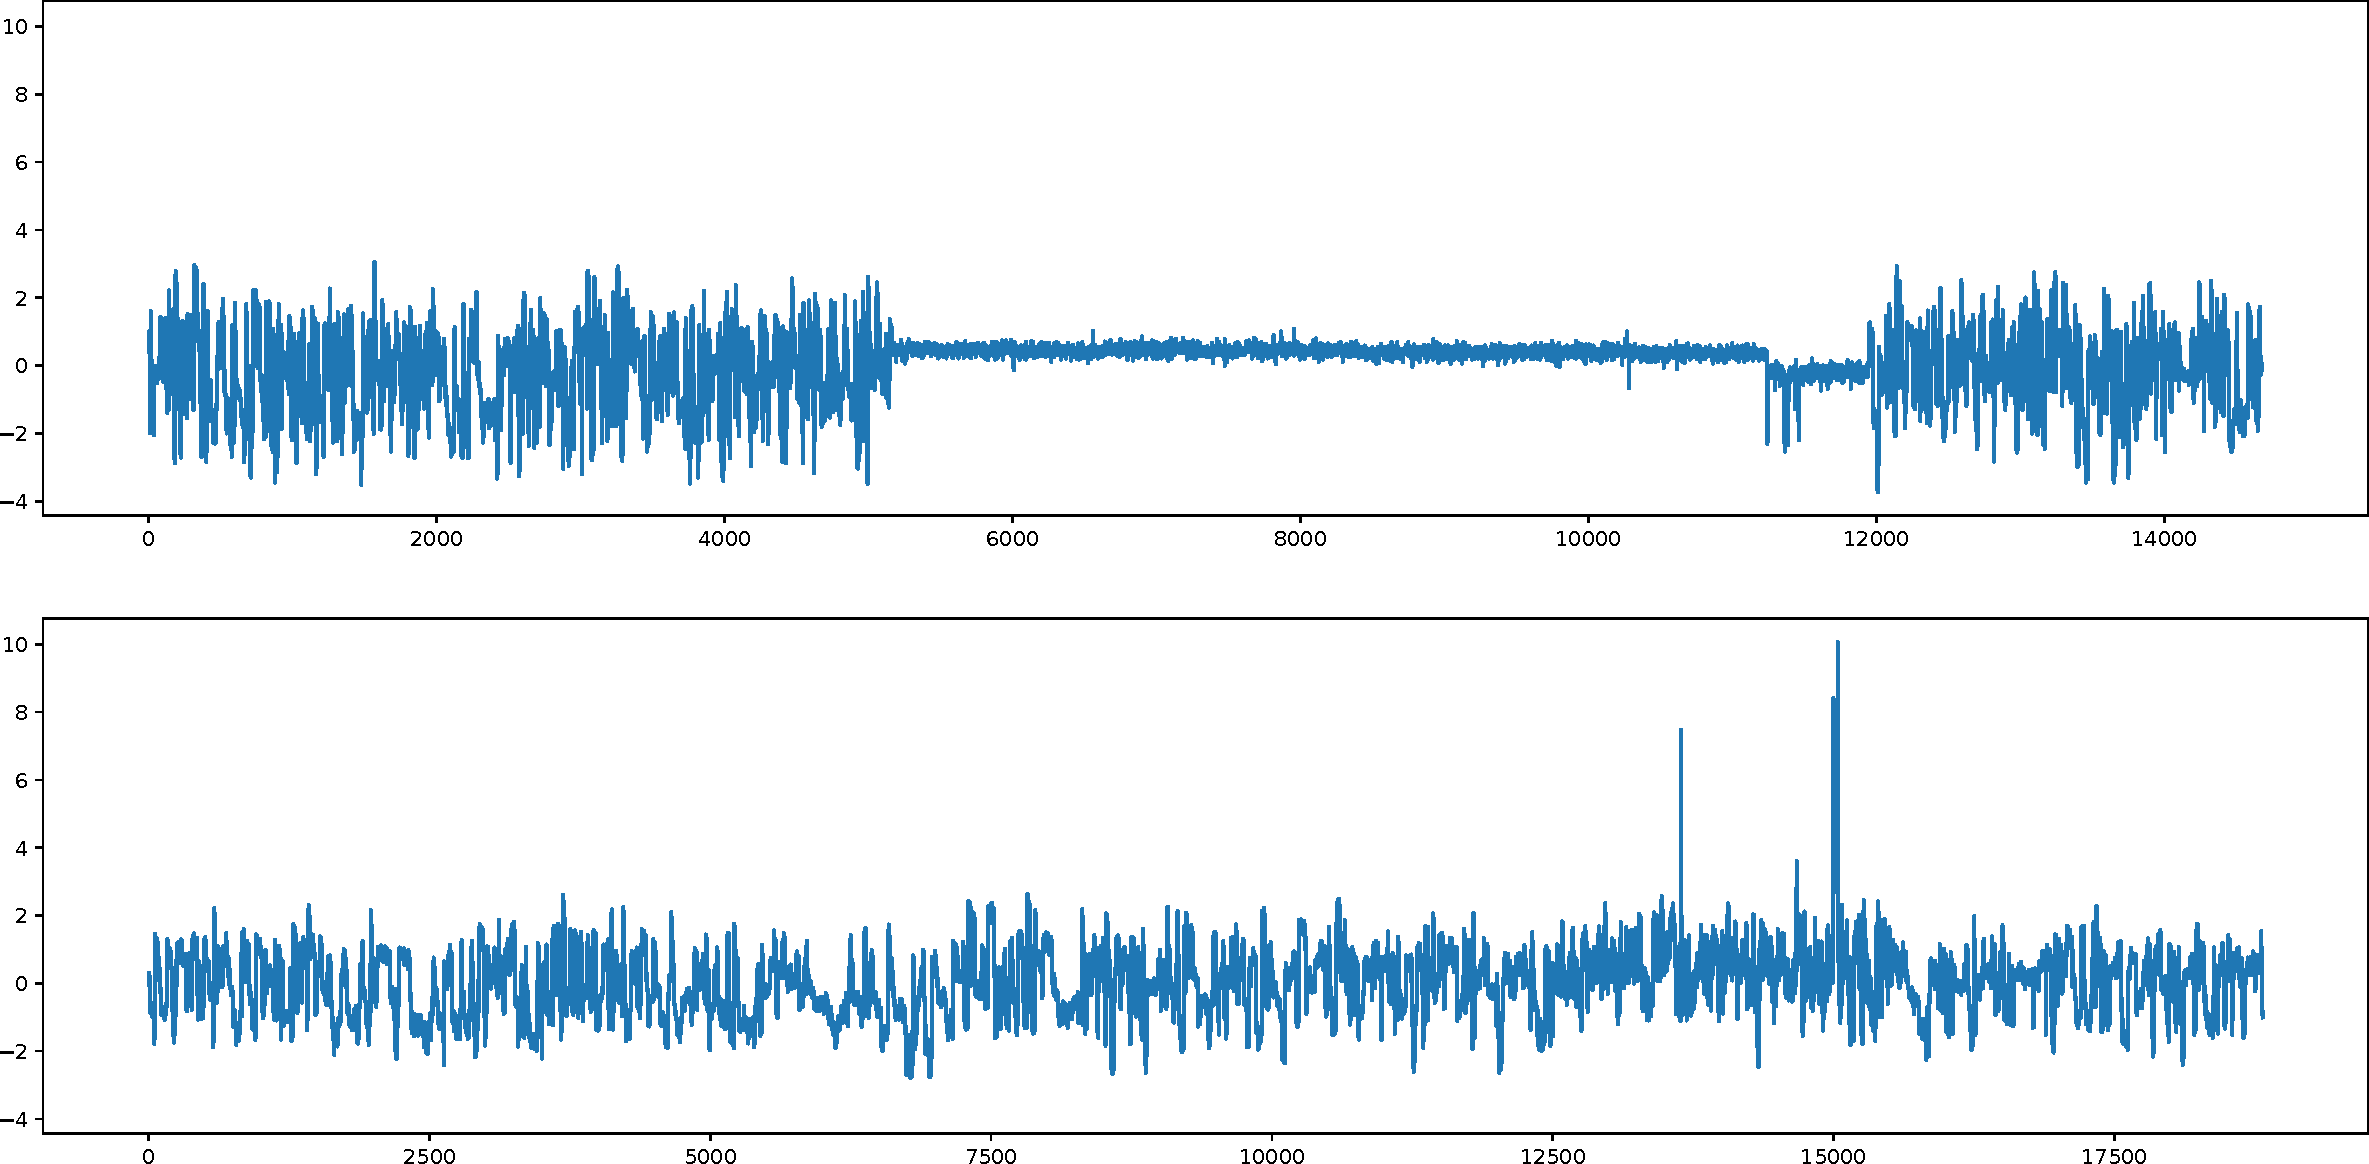
\includegraphics[width=1.0\textwidth]{images/signals}
  \caption{Defect data found by simple visualization.}
  \label{fig:signals}
\end{figure}

\section{Alignment}
TODO: something like \ref{fig:pairing} and \ref{fig:foos}

\begin{figure}[h]
  \centering
  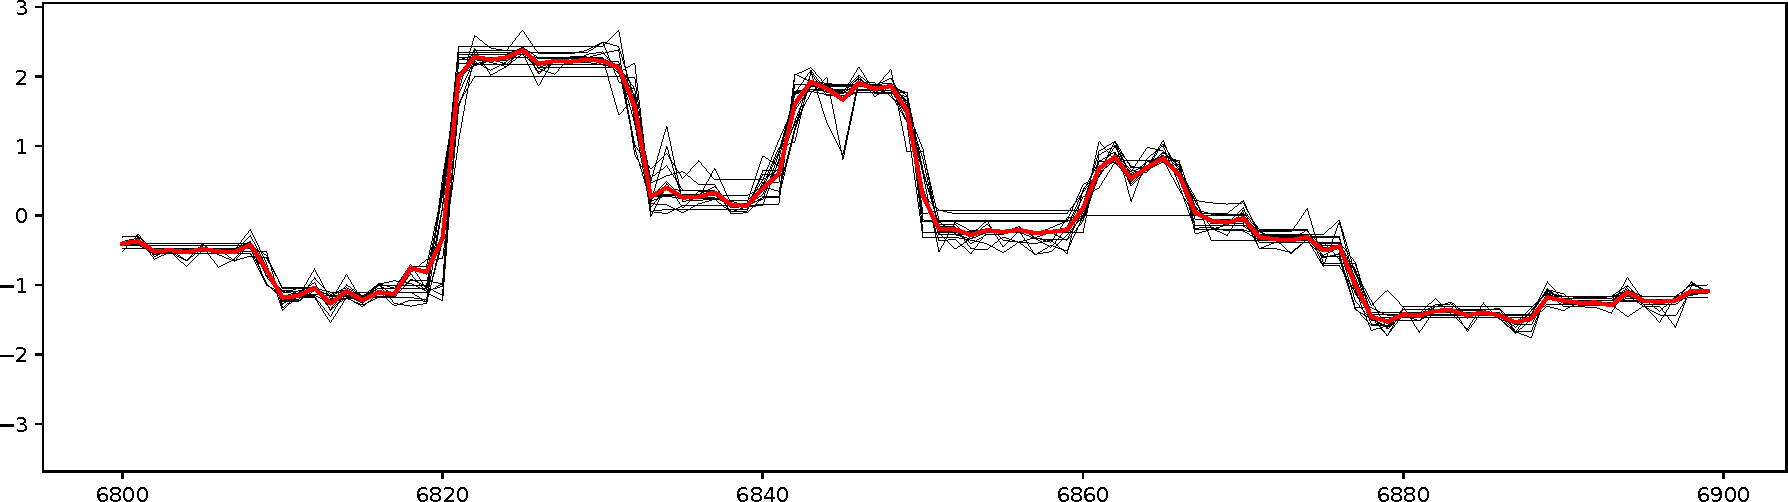
\includegraphics[width=1.0\textwidth]{images/foos}
  \caption{Some caption.}
  \label{fig:foos}
\end{figure}